\documentclass[14pt, a4paper]{extarticle}

\usepackage[margin=1in]{geometry}
\usepackage{graphicx}
\usepackage{enumitem}
\usepackage{multicol}
\usepackage{fancyhdr}
\usepackage{amsfonts}
\usepackage{amssymb}
\usepackage{listings}
\usepackage{float}
\usepackage{wrapfig}

\usepackage{gvv-book}
\usepackage{gvv}

\graphicspath{ {figs/} }

\pagestyle{fancy}
\fancyhf{} 
\fancyhead[L]{2009}
\fancyhead[R]{PH}
\fancyfoot[L]{PH}
\fancyfoot[R]{\thepage/20}
\renewcommand{\headrulewidth}{0.4pt}
\renewcommand{\footrulewidth}{0.4pt}

\let\oldvec\vec
\renewcommand{\vec}[1]{\overrightarrow{#1}}
\newcommand{\myvec}[1]{\begin{bmatrix} #1 \end{bmatrix}}



\begin{document}

\begin{center}
    
    {\Large \underline{\textbf{Some Useful Constants}}}
    \vspace{1em}
   
    \begin{tabular}{l @{ : }  l}
        Speed of light constant & $c$ \\
        Boltzmann constant & $k_B$ \\
        Electron charge & $e$ \\
        Planck's constant & $h$ \\
        Rest mass of electron & $m_e$ \\
        Rest mass of proton & $m_p$ \\
        Permeability of free space & $\mu_0$ \\
        Permittivity of free space & $\varepsilon_0$ \\
    \end{tabular}
    
    \vspace{1.5em}
    
    All other symbols have their usual meanings unless otherwise specified.
    
\end{center}

\vspace{1em}
\noindent
\textbf{Q. 1 -- Q. 20 carry one mark each}

\begin{enumerate}[label=\textbf{Q. \arabic*}]

\item The value of the contour integral
    $ \left| \oint_C \vec{r} \times d\vec{\theta} \right| $,
    for a circle $C$ of radius $r$ with center at the origin is:
    \begin{enumerate}
    \begin{multicols}{4}
        \item $2\pi r$
        \item $\dfrac{r^2}{2}$
        \item $\pi r^2$
        \item $r$
    \end{multicols}
    \end{enumerate}
    \hfill \textbf{(GATE PH 2009)}

\item An electrostatic field $\vec{E}$ exists in a given region $R$. Choose the \textbf{wrong} statement.
   
    \begin{enumerate}
        \item Circulation of $\vec{E}$ is zero.
        \item $\vec{E}$ can always be expressed as the gradient of a scalar field.
        \item The potential difference between any two arbitrary points in the region R is zero.
        \item The work done in a closed path lying entirely in $R$ is zero.   
    \end{enumerate}
    \hfill \textbf{(GATE PH 2009)}


\item The Lagrangian of a free particle in spherical polar co-ordinates is given by
    \begin{align*}
    L = \frac{1}{2}m(\dot{r}^2 + r^2\dot{\theta}^2 + r^2\sin^2\theta\dot{\phi}^2)
    \end{align*}
    The quantity that is conserved is:
    \begin{multicols}{2}
    \begin{enumerate}
        \item $\dfrac{\partial L}{\partial \dot{r}}$
        \item $\dfrac{\partial L}{\partial \dot{\theta}}$
        \item $\dfrac{\partial L}{\partial \dot{\phi}}$
        \item $\dfrac{\partial L}{\partial \dot{\phi}} + r \dot{\theta}$
    \end{enumerate}
    \end{multicols}
    \hfill \textbf{(GATE PH 2009)}

\item A conducting loop L of surface area S is moving with a velocity $\vec{v}$ in a magnetic field $\vec{B}(\vec{r}, t) = B_o t^2 \hat{z}$.
$B_o$ is a positive constant of suitable dimensions. The emf induced, $V_{\text{emf}}$, in the loop is given by
\begin{multicols}{2}
\begin{enumerate}
\item $-\int_S \dfrac{\partial\vec{B}}{\partial t} \cdot d\vec{S}$
\item $\oint_L (\vec{v} \times \vec{B}) \cdot d\vec{L}$
\item $-\int_S \dfrac{\partial\vec{B}}{\partial t} \cdot d\vec{S} - \oint_L (\vec{v} \times \vec{B}) \cdot d\vec{L}$
\item $-\int_S \dfrac{\partial\vec{B}}{\partial t} \cdot d\vec{S} + \oint_L (\vec{v} \times \vec{B}) \cdot d\vec{L}$
\end{enumerate}
\end{multicols}
\hfill \textbf{(GATE PH 2009)}

\item The eigenvalues of the matrix $\vec{A} = \myvec{0 & i \\ i & 0}$ are
    \begin{multicols}{2}
    \begin{enumerate}
        \item real and distinct
        \item complex and distinct
        \item complex and coinciding
        \item real and coinciding
    \end{enumerate}
    \end{multicols}
    \hfill \textbf{(GATE PH 2009)}
    

\item $\sigma_i (i=1, 2, 3)$ represent the Pauli spin matrices. Which one of the following is \textbf{NOT} true?
    \begin{multicols}{2}
    \begin{enumerate}
        \item $\sigma_i \sigma_j + \sigma_j \sigma_i = 2\delta_{ij}$
        \item $\operatorname{Tr}(\sigma_i) = 0$
        \item The eigenvalues of $\sigma_i$ are $\pm 1$
        \item $\det(\sigma_i) = 1$
    \end{enumerate}
    \end{multicols}
    \hfill \textbf{(GATE PH 2009)}

\item Which one of the functions given below represents the bound state eigenfunction of the operator $-\dfrac{d^2}{dx^2}$ in the region, $0 \le x < \infty$, with the eigenvalue $-4$\,?
    \begin{multicols}{2}
    \begin{enumerate}
        \item $A_o e^{2x}$
        \item $A_o \cosh 2x$
        \item $A_o e^{-2x}$
        \item $A_o \sinh 2x$
    \end{enumerate}
    \end{multicols}
    \hfill \textbf{(GATE PH 2009)}

\item Pick the \textbf{WRONG} statement.
    \begin{enumerate}
        \item The nuclear force is independent of electric charge
        \item The Yukawa potential is proportional to $r^{-1} \exp\left(-\dfrac{mc}{\hbar} r\right)$, where r is the separation between two nucleons
        \item The range of nuclear force is of the order of $10^{-15}\,\mathrm{m} - 10^{-14}\,\mathrm{m}$
        \item The nucleons interact among each other by the exchange of mesons
    \end{enumerate}
    \hfill \textbf{(GATE PH 2009)}

\item If p and q are the position and momentum variables, which one of the following is \textbf{NOT} a canonical transformation?
    \begin{enumerate}
        \item $Q = \alpha q$ and $P = \dfrac{1}{\alpha}p$, for $\alpha \neq 0$
        \item $Q = \alpha q + \beta p$ and $P = \beta q + \alpha p$ for $\alpha, \beta$ real and $\alpha^2 - \beta^2 = 1$
        \item $Q = p$ and $P = q$
        \item $Q = p$ and $P = -q$
    \end{enumerate}
    \hfill \textbf{(GATE PH 2009)}

\item The Common Mode Rejection Ratio (CMRR) of a differential amplifier using an operational amplifier is 100 dB.
The output voltage for a differential input of $200\,\mu\text{V}$ is 2 V. The common mode gain is
\begin{enumerate}
\begin{multicols}{2}
\item 10
\item 0.1
\item 30 dB
\item 10 dB
\end{multicols}
\end{enumerate}
\hfill \textbf{(GATE PH 2009)}

\item In an insulating solid which one of the following physical phenomena is a consequence of Pauli's exclusion principle?
    \begin{enumerate}
        \item Ionic conductivity
        \item Ferromagnetism
        \item Paramagnetism
        \item Ferroelectricity
    \end{enumerate}
    \hfill \textbf{(GATE PH 2009)}

\item Which one of the following curves gives the solution of the differential equation
$ k_1\dfrac{dx}{dt} + k_2x = k_3, $
where $k_1, k_2$ and $k_3$ are positive constants with initial conditions $x=0$ at $t=0$?
\begin{enumerate}
\begin{multicols}{2}
\item 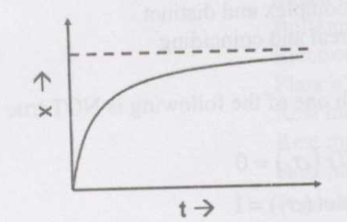
\includegraphics[width=0.9\columnwidth]{graphA.png}
\item 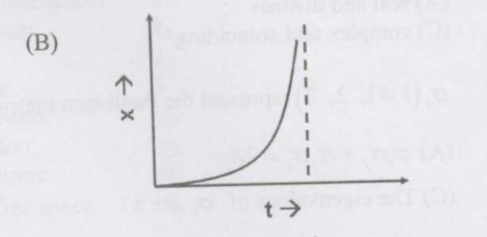
\includegraphics[width=0.9\columnwidth]{graphB.png}
\item 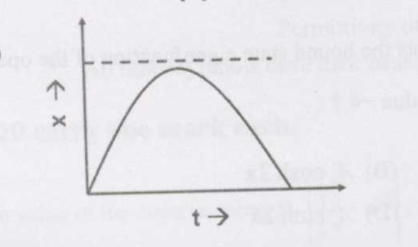
\includegraphics[width=0.9\columnwidth]{graphC.png}
\item 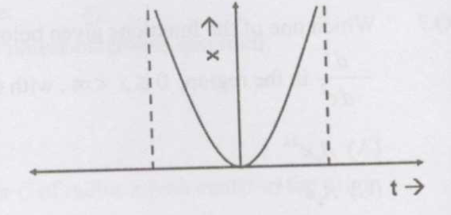
\includegraphics[width=0.9\columnwidth]{graphD.png}
\end{multicols}
\end{enumerate}
\hfill \textbf{(GATE PH 2009)}

\item Identify which one is a first order phase transition?
    \begin{enumerate}
        \item A liquid to gas transition at its critical temperature.
        \item A liquid to gas transition close to its triple point.
        \item A paramagnetic to ferromagnetic transition in the absence of a magnetic field.
        \item A metal to superconductor transition in the absence of a magnetic field.
    \end{enumerate}
    \hfill \textbf{(GATE PH 2009)}

\item Group I lists some physical phenomena while Group II gives some physical parameters. Match the phenomena with the corresponding parameter.
    \begin{center}
    \begin{multicols}{2}
        \textbf{Group I}
        \begin{itemize}
            \item[P.] Doppler Broadening
            \item[Q.] Natural Broadening
            \item[R.] Rotational spectrum
            \item[S.] Total internal reflection
        \end{itemize}
        \textbf{Group II}
        \begin{itemize}
            \item[1.] Moment of inertia
            \item[2.] Refractive index
            \item[3.] Lifetime of the energy level
            \item[4.] Pressure
        \end{itemize}
    \end{multicols}
    \end{center}
    \begin{enumerate}
        \item P-4, Q-3, R-1, S-2
        \item P-3, Q-2, R-1, S-4
        \item P-2, Q-3, R-4, S-1
        \item P-1, Q-4, R-2, S-3
    \end{enumerate}
    \hfill \textbf{(GATE PH 2009)}

\item The separation between the first Stokes and corresponding anti-Stokes lines of the rotational Raman spectrum in terms of the rotational constant, B is
    \begin{enumerate}
    \begin{multicols}{4}
        \item 2$B$
        \item 4$B$
        \item 6$B$
        \item 12$B$
    \end{multicols}
    \end{enumerate}
    \hfill \textbf{(GATE PH 2009)}

\item A superconducting ring is cooled in the presence of a magnetic field below its critical temperature ($T_C$). 
The total magnetic flux that passes through the ring is
\begin{enumerate}
\begin{multicols}{2}
\item zero
\item $n \dfrac{h}{2e}$
\item $\dfrac{nh}{4\pi e}$
\item $\dfrac{ne^2}{hc}$
\end{multicols}
\end{enumerate}
\hfill \textbf{(GATE PH 2009)}

\item In a cubic crystal, atoms of mass $M_1$ lie on one set of planes and atoms of mass $M_2$ lie on planes interleaved between those of the first set. If $C$ is the force constant between nearest neighbour planes, the frequency of lattice vibrations for the optical phonon branch with wavevector $k=0$ is
\begin{enumerate}
\item$\; \sqrt{\,2C \left(\dfrac{1}{M_1} + \dfrac{1}{M_2}\right)}$
\item$\; \sqrt{\,C \left(\dfrac{1}{2M_1} + \dfrac{1}{M_2}\right)}$
\item$\; \sqrt{\,C \left(\dfrac{1}{M_1} + \dfrac{1}{2M_2}\right)}$
\item$\; 0$
\end{enumerate}
\hfill \textbf{(GATE PH 2009)}

\item In the quark model which one of the following represents a proton?
    \begin{enumerate}
    \begin{multicols}{4}
        \item $udd$
        \item $uud$
        \item $u\bar{b}$
        \item $c\bar{c}$
    \end{multicols}
    \end{enumerate}
    \hfill \textbf{(GATE PH 2009)}

\item

\begin{figure}[H]
\centering
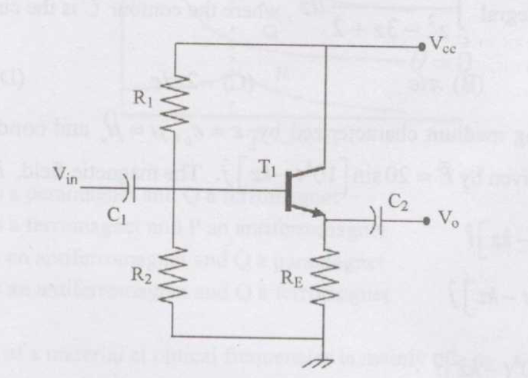
\includegraphics[width=0.6\columnwidth]{figs/Q19fig.png}
\caption{Circuit diagram}
\label{fig:q17}
\end{figure}

The circuit shown above
\begin{enumerate}
\begin{multicols}{2}
\item is a common-emitter amplifier
\item uses a pnp transistor
\item is an oscillator
\item has a voltage gain less than one
\end{multicols}
\end{enumerate}
\hfill \textbf{(GATE PH 2009)}

\item Consider a nucleus with N neutrons and Z protons. If $m_p$, $m_n$ and BE represent the mass of the proton, the mass of the neutron and the binding energy of the nucleus respectively and $c$ is the velocity of light in free space, the mass of the nucleus is given by
    \begin{enumerate}
    \begin{multicols}{2}
        \item $Nm_n + Zm_p$
        \item $Nm_p + Zm_n$
        \item $Nm_n + Zm_p + \dfrac{BE}{c^2}$
        \item $Nm_p + Zm_n + \dfrac{BE}{c^2}$
    \end{multicols}
    \end{enumerate}
\end{enumerate}
\hfill \textbf{(GATE PH 2009)}

\vspace{1.5em}
\noindent 
\textbf{Q. 21 to Q. 60 carry two marks each.}
\vspace{1em}

\begin{enumerate}[label=\textbf{Q. \arabic*}, start=21]

\item The magnetic field (in $A~m^{-1}$) inside a long solid cylindrical conductor of radius $a = 0.1$ m is,
$ \vec{H} = \dfrac{10^4}{r} \left[ \dfrac{1}{\alpha^2}\sin(\alpha r) - \dfrac{r}{\alpha}\cos(\alpha r) \right] \hat{\phi}, \quad \text{where } \alpha = \dfrac{\pi}{2a}. $
What is the total current (in A) in the conductor?
\begin{enumerate}
\begin{multicols}{4}
\item $\dfrac{\pi}{2a}$
\item $\dfrac{800}{\pi}$
\item $\dfrac{400}{\pi}$
\item $\dfrac{300}{\pi}$
\end{multicols}
\end{enumerate}
\hfill \textbf{(GATE PH 2009)}

\item Which one of the following current densities, $\vec{J}$, can generate the magnetic vector potential $\vec{A} = (y^2\hat{i} + x^2\hat{j})$?
\begin{enumerate}
\begin{multicols}{2}
\item $\dfrac{2}{\mu_0}(x\hat{i} + y\hat{j})$
\item $-\dfrac{2}{\mu_0}(\hat{i} + \hat{j})$
\item $\dfrac{2}{\mu_0}(\hat{i} - \hat{j})$
\item $\dfrac{2}{\mu_0}(x\hat{i} - y\hat{j})$
\end{multicols}
\end{enumerate}
\hfill \textbf{(GATE PH 2009)}

\item The value of the integral $\oint_C \dfrac{e^z}{z^2 - 3z + 2} dz,$
where the contour $C$ is the circle $|z| = 3/2$ is
\begin{enumerate}
\begin{multicols}{4}
\item $2\pi i e$
\item $\pi i e$
\item $-2\pi i e$
\item $-\pi i e$
\end{multicols}
\end{enumerate}
\hfill \textbf{(GATE PH 2009)}

\item In a non-conducting medium characterized by $\varepsilon = \varepsilon_0$, $\mu = \mu_o$ and conductivity $\sigma = 0$, the electric field (in $V~m^{-1}$) is given by $\vec{E} = 20\sin[10^8 t - kz] \hat{j}$. The magnetic field, $\vec{H}$ (in $A~m^{-1}$), is given by
\begin{enumerate}
\item $20k \cos[10^8 t - kz] \hat{i}$
\item $\dfrac{20k}{10^8 \mu_o}\sin[10^8 t - kz] \hat{j}$
\item $-\dfrac{20k}{10^8 \mu_o}\sin[10^8 t - kz] \hat{i}$
\item $-20k \cos[10^8 t - kz] \hat{j}$
\end{enumerate}
\hfill \textbf{(GATE PH 2009)}

\item A cylindrical rod of length $L$ and radius $r$, made of an inhomogeneous dielectric, is placed with its axis along the $z$ direction with one end at the origin as shown below.
\begin{figure}[H]
\centering
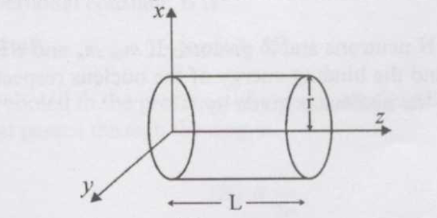
\includegraphics[width=0.4\textwidth]{figs/Q25fig.png}
\caption{Cylindrical rod of length $L$ and radius $r$ }
\label{fig:q25}
\end{figure}
If the rod carries a polarization, $\vec{P} = (5z^2 + 7)\hat{k}$, the volume bound charge inside the dielectric is
\begin{enumerate}
\begin{multicols}{4}
\item Zero
\item $10\pi r^2 L$
\item $-5\pi r^2 L$
\item $-5\pi r^2 L^2$
\end{multicols}
\end{enumerate}
\hfill \textbf{(GATE PH 2009)}

\item Let $T_{ij} = \sum_k \varepsilon_{ijk} a_k$ and $\beta_k = \sum_{i,j} \varepsilon_{ijk} T_{ij}$, where $\varepsilon_{ijk}$ is the Levi-Civita density, defined to be zero if two of the indices coincide and $+1$ and $-1$ depending on whether $ijk$ is even or odd permutation of $1,2,3$. Then $\beta_3$ is equal to
\begin{enumerate}
\begin{multicols}{4}
\item $2a_3$
\item $-2a_3$
\item $a_3$
\item $-a_3$
\end{multicols}
\end{enumerate}
\hfill \textbf{(GATE PH 2009)}

\item The dependence of the magnetic susceptibility ($\chi$) of a material with temperature (T) can be represented by $\chi \propto \frac{1}{T-\theta}$, where $\theta$ is the Curie-Weiss temperature.
The plot of magnetic susceptibility versus temperature is sketched in the figure, as curves P, Q and R with curve Q having $\theta=0$.
Which one of the following statements is correct?
\begin{figure}[H]
\centering
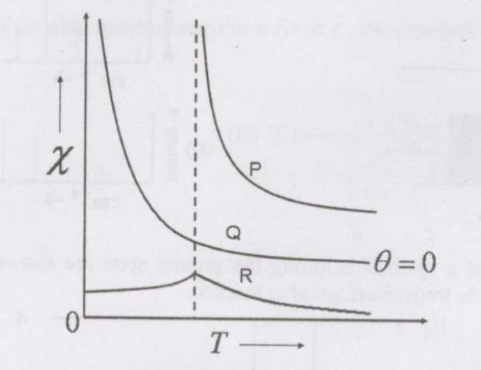
\includegraphics[width=0.5\columnwidth]{figs/Q27figs.png}
\caption{Magnetic susceptibility ($\chi$) of a material vs. Temperature}
\label{fig:q27}
\end{figure}
\begin{enumerate}
\item Curve R represents a paramagnet and Q a ferromagnet
\item Curve Q represents a ferromagnet and P an antiferromagnet
\item Curve R represents an antiferromagnet and Q a paramagnet
\item Curve R represents an antiferromagnet and Q a ferromagnet
\end{enumerate}
\hfill \textbf{(GATE PH 2009)}

\item The dielectric constant of a material at optical frequencies is mainly due to
\begin{enumerate}
\begin{multicols}{2}
\item ionic polarizability
\item electronic polarizability
\item dipolar polarizability
\item ionic and dipolar polarizability
\end{multicols}
\end{enumerate}
\hfill \textbf{(GATE PH 2009)}

\item An electron of wavevector $\vec{k}_e$, velocity $\vec{v}_e$ and effective mass $m_e$ is removed from a filled energy band. The resulting hole has wavevector $\vec{k}_h$, velocity $\vec{v}_h$ and effective mass $m_h$. Which one of the following statements is correct?
\begin{enumerate}
\item $\vec{k}_h = -\vec{k}_e; \quad \vec{v}_h = -\vec{v}_e; \quad m_h = -m_e$
\item $\vec{k}_h = \vec{k}_e; \quad \vec{v}_h = \vec{v}_e; \quad m_h = m_e$
\item $\vec{k}_h = \vec{k}_e; \quad \vec{v}_h = -\vec{v}_e; \quad m_h = -m_e$
\item $\vec{k}_h = -\vec{k}_e; \quad \vec{v}_h = \vec{v}_e; \quad m_h = -m_e$
\end{enumerate}
\hfill \textbf{(GATE PH 2009)}

\vspace{24em}

\item In a diatomic molecule, the internuclear separation of the ground and first excited electronic state are the same as shown in the figure.
If the molecule is initially in the lowest vibrational state of the ground state, then the absorption spectrum will appear as
\begin{figure}[H]
\centering
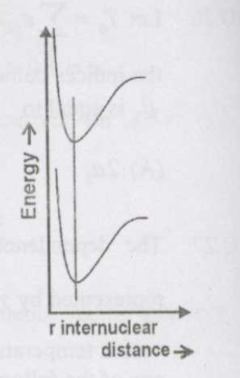
\includegraphics[width=0.4\textwidth]{figs/Q30fig1.png}
\caption{Potential energy curves for a diatomic molecule}
\label{fig:q30_main}
\end{figure}
\begin{enumerate}
\begin{multicols}{2}
\item 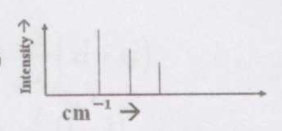
\includegraphics[width=0.4\textwidth]{figs/Q30fig2.png}

\item 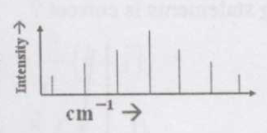
\includegraphics[width=0.4\textwidth]{figs/Q30fig3.png}

\item 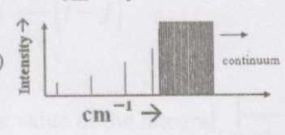
\includegraphics[width=0.4\textwidth]{figs/Q30fig4.png}

\item 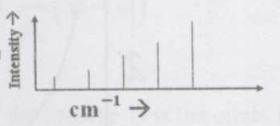
\includegraphics[width=0.4\textwidth]{figs/Q30fig5.png}

\end{multicols}
\end{enumerate}
\hfill \textbf{(GATE PH 2009)}

\vspace{12em}

\item Five energy levels of a system including the ground state are shown below.
Their lifetimes and the allowed electric dipole transitions are also marked.
\begin{figure}[H]
\centering
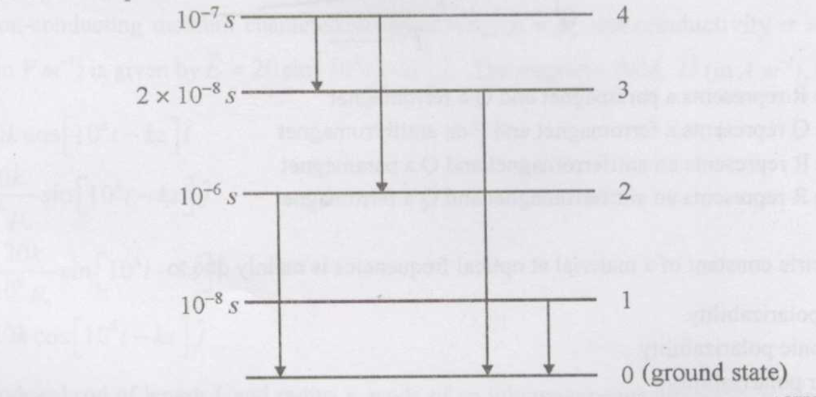
\includegraphics[width=0.6\textwidth]{figs/Q31fig.png}
\caption{Energy levels of a system}
\label{fig:q31}
\end{figure}
Which one of the following transitions is the most suitable for a continuous wave (CW) laser?
\begin{enumerate}
\begin{multicols}{4}
\item $1 \rightarrow 0$
\item $2 \rightarrow 0$
\item $4 \rightarrow 2$
\item $4 \rightarrow 3$
\end{multicols}
\end{enumerate}
\hfill \textbf{(GATE PH 2009)}

\item Assuming the mean life time of a muon (in its rest frame) to be $2\times10^{-6}$ s, its life time in the laboratory frame, when it is moving with a velocity $0.95c$ is
    \begin{enumerate}
    \begin{multicols}{2}
        \item $6.4\times10^{-6}$ s
        \item $0.62\times10^{-6}$ s
        \item $2.16\times10^{-6}$ s
        \item $0.19\times10^{-6}$ s
    \end{multicols}
    \end{enumerate}
    \hfill \textbf{(GATE PH 2009)}


\item Cesium has a nuclear spin of $7/2$. The hyperfine spectrum of the D lines of the cesium atom will consist of
\begin{enumerate}
\begin{multicols}{4}
\item 10 lines
\item 4 lines
\item 6 lines
\item 14 lines
\end{multicols}
\end{enumerate}
\hfill \textbf{(GATE PH 2009)}

\item The probability that an energy level $\varepsilon$ at a temperature $T$ is unoccupied by a fermion of chemical potential $\mu$ is given by
\begin{enumerate}
\item $\dfrac{1}{e^{(\varepsilon-\mu)/k_B T} + 1}$
\item $\dfrac{1}{e^{(\varepsilon-\mu)/k_B T} - 1}$
\item $\dfrac{1}{e^{(\mu-\varepsilon)/k_B T} + 1}$
\item $\dfrac{1}{e^{(\mu-\varepsilon)/k_B T} - 1}$
\end{enumerate}
\hfill \textbf{(GATE PH 2009)}

\item Consider the following expression for the mass of a nucleus with Z protons and A nucleons:
$M(A,Z) = \dfrac{1}{c^2}(f(A) + yZ + zZ^2)$
Here $f(A)$ is a function of A,
\begin{align*}
& y = -4a_A, \\
& z = a_c A^{-1/3} + 4a_A A^{-1},
\end{align*}
$a_A$ and $a_c$ are constants of suitable dimensions. For a fixed A, the expression of Z for the most stable nucleus is
\begin{enumerate}
\begin{multicols}{2}
\item $Z = \dfrac{A/2}{1 + \left( \dfrac{a_c}{a_A} \right) A^{2/3}}$
\item $Z = \dfrac{A/2}{1 + \left( \dfrac{a_c}{4a_A} \right) A^{2/3}}$
\item $Z = \dfrac{A}{1 + \left( \dfrac{a_c}{4a_A} \right) A^{2/3}}$
\item $Z = \dfrac{A}{1 + A^{2/3}}$
\end{multicols}
\end{enumerate}
\hfill \textbf{(GATE PH 2009)}

\item The de Broglie wavelength of particles of mass $m$ with average momentum $p$ at a temperature $T$ in three dimensions is given by
\begin{enumerate}
\begin{multicols}{2}
\item $\lambda = \dfrac{h}{\sqrt{2mk_B T}}$
\item $\lambda = \dfrac{h}{\sqrt{3mk_B T}}$
\item $\lambda = \dfrac{h}{\sqrt{2k_B T}}$
\item $\lambda = \dfrac{h}{\sqrt{3m}}$
\end{multicols}
\end{enumerate}
\hfill \textbf{(GATE PH 2009)}

\vspace{14em}

\item \leavevmode \par
    \begin{center}
        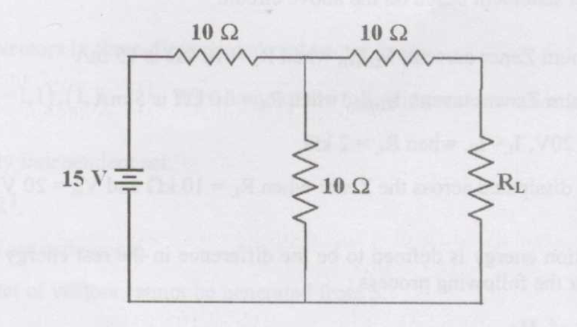
\includegraphics[width=0.6\columnwidth]{figs/Q37fig.png}
        \captionof{figure}{Circuit for Question 37.}
        \label{fig:q37}
    \end{center}
Assuming an ideal voltage source, Thevenin's resistance and Thevenin's voltage respectively for the above circuit are
\begin{enumerate}
\begin{multicols}{2}
\item $15\,\Omega$ and $7.5$ V
\item $20\,\Omega$ and $5$ V
\item $10\,\Omega$ and $10$ V
\item $30\,\Omega$ and $15$ V
\end{multicols}
\end{enumerate}
\hfill \textbf{(GATE PH 2009)}

\item Let $|n\rangle$ and $|p\rangle$ denote the isospin states with $I = 1/2$, $I_3 = 1/2$ and $I = 1/2$, $I_3 = -1/2$ of a nucleon respectively. Which one of the following two-nucleon states has $I=0, I_3=0$?
\begin{enumerate}
\begin{multicols}{2}
\item $\dfrac{1}{\sqrt{2}}(|nn\rangle - |pp\rangle)$
\item $\dfrac{1}{\sqrt{2}}(|nn\rangle + |pp\rangle)$
\item $\dfrac{1}{\sqrt{2}}(|np\rangle - |pn\rangle)$
\item $\dfrac{1}{\sqrt{2}}(|np\rangle + |pn\rangle)$
\end{multicols}
\end{enumerate}
\hfill \textbf{(GATE PH 2009)}

\item An amplifier of gain 1000 is made into a feedback amplifier by feeding 9.9\,\% of its output voltage in series with the input opposing. If $f_L = 20\,\text{Hz}$ and $f_H = 200\,\text{kHz}$ for the amplifier without feedback, then due to the feedback [cite: 8]
    \begin{enumerate}
    \begin{multicols}{2}
        \item the gain decreases by 10 times [cite: 8]
        \item the output resistance increases by 10 times [cite: 8]
        \item the $f_H$ increases by 100 times [cite: 8]
        \item the input resistance decreases by 100 times [cite: 8]
    \end{multicols}
    \end{enumerate}
    \hfill \textbf{(GATE PH 2009)}

\item \leavevmode \par
    \begin{center}
        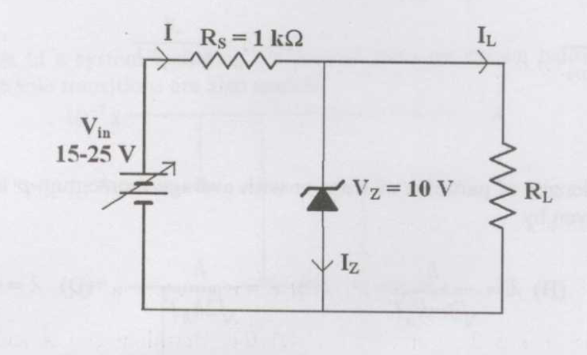
\includegraphics[width=0.6\columnwidth]{figs/Q40fig.png}
        \captionof{figure}{Circuit for Question 40.}
        \label{fig:q40}
    \end{center}
Pick the correct statement based on the above circuit.
\begin{enumerate}
\item The maximum Zener current, $I_{z(\max)}$, when $R_L = 10\,\text{k}\Omega$ is $15\,\text{mA}$
\item The minimum Zener current, $I_{z(\min)}$, when $R_L = 10\,\text{k}\Omega$ is $5\,\text{mA}$
\item With $V_{\text{in}} = 20\,\text{V}$, $I_L = I_Z$, when $R_L = 2\,\text{k}\Omega$
\item The power dissipated across the Zener when $R_L = 10\,\text{k}\Omega$ and $V_{\text{in}} = 20\,\text{V}$ is $100\,\text{mW}$
\end{enumerate}
\hfill \textbf{(GATE PH 2009)}


\item The disintegration energy is defined to be the difference in the rest energy between the initial and final states.
Consider the following process:
\begin{align*} ^{240}_{94}\text{Pu} \rightarrow ^{236}_{92}\text{U} + ^{4}_{2}\text{He}. \end{align*}
The emitted $\alpha$ particle has a kinetic energy 5.17 MeV. The value of the disintegration energy is
\begin{enumerate}
\begin{multicols}{4}
\item 5.26 MeV
\item 5.17 MeV
\item 5.08 MeV
\item 2.59 MeV
\end{multicols}
\end{enumerate}
\hfill \textbf{(GATE PH 2009)}

\item A classical particle is moving in an external potential field $V(x,y,z)$ which is invariant under the following infinitesimal transformations
\begin{align*}
& x \rightarrow x' = x + \delta x, \\
& y \rightarrow y' = y + \delta y, \\
& \begin{pmatrix} x \\ y \end{pmatrix} \rightarrow \begin{pmatrix} x' \\ y' \end{pmatrix} = R_z \begin{pmatrix} x \\ y \end{pmatrix},
\end{align*}
where $R_z$ is the matrix corresponding to rotation about the z axis.
The conserved quantities are (the symbols have their usual meaning)
\begin{enumerate}
\begin{multicols}{4}
\item $p_x, p_z, L_z$
\item $p_x, p_y, L_z, E$
\item $p_y, L_z, E$
\item $p_y, p_z, L_z, E$
\end{multicols}
\end{enumerate}
\hfill \textbf{(GATE PH 2009)}

\item The spin function of a free particle, in the basis in which $S_z$ is diagonal, can be written as
$\begin{pmatrix} 1 \\ 0 \end{pmatrix}$ and $\begin{pmatrix} 0 \\ 1 \end{pmatrix}$ with eigenvalues $+\dfrac{\hbar}{2}$ and $-\dfrac{\hbar}{2}$, respectively. In the given basis, the normalized eigenfunction of $S_y$ with eigenvalue $-\dfrac{\hbar}{2}$ is
\begin{enumerate}
\begin{multicols}{4}
\item $\dfrac{1}{\sqrt{2}}\begin{pmatrix} 1 \\ i \end{pmatrix}$
\item $\dfrac{1}{\sqrt{2}}\begin{pmatrix} 0 \\ i \end{pmatrix}$
\item $\dfrac{1}{\sqrt{2}}\begin{pmatrix} i \\ 0 \end{pmatrix}$
\item $\dfrac{1}{\sqrt{2}}\begin{pmatrix} 1 \\ i \end{pmatrix}$
\end{multicols}
\end{enumerate}
\hfill \textbf{(GATE PH 2009)}

\item $\hat{A}$ and $\hat{B}$ represent two physical characteristics of a quantum system. If $\hat{A}$ is Hermitian, then for the product $\hat{A}\hat{B}$ to be Hermitian, it is sufficient that
\begin{enumerate}
\begin{multicols}{2}
\item $\hat{B}$ is Hermitian
\item $\hat{B}$ is anti-Hermitian
\item $\hat{B}$ is Hermitian and $\hat{A}$ and $\hat{B}$ commute
\item $\hat{B}$ is Hermitian and $\hat{A}$ and $\hat{B}$ anti-commute
\end{multicols}
\end{enumerate}
\hfill \textbf{(GATE PH 2009)}

\item Consider the set of vectors in three-dimensional real vector space $\mathbf{R}^3, S = \{(1,1,1), (1,-1,1), (1,1,-1)\}$. Which one of the following statements is true?
\begin{enumerate}
\item $S$ is not a linearly independent set.
\item $S$ is a basis for $\mathbf{R}^3$.
\item The vectors in $S$ are orthogonal.
\item An orthogonal set of vectors cannot be generated from $S$.
\end{enumerate}
\hfill \textbf{(GATE PH 2009)}

\item For a Fermi gas of $N$ particles in three dimensions at $T=0$ K, the Fermi energy, $E_F$, is proportional to
\begin{enumerate}
\begin{multicols}{4}
\item $N^{2/3}$
\item $N^{3/2}$
\item $N^3$
\item $N^2$
\end{multicols}
\end{enumerate}
\hfill \textbf{(GATE PH 2009)}

\item The Lagrangian of a diatomic molecule is given by $L = \dfrac{m}{2}(\dot{x}_1^2 + \dot{x}_2^2) - \dfrac{k}{2}x_1 x_2$, where $m$ is the mass of each of the atoms and $x_1$ and $x_2$ are the displacements of atoms measured from the equilibrium position and $k > 0$. The normal frequencies are
\begin{enumerate}
\begin{multicols}{4}
\item $\pm \left( \dfrac{k}{m} \right)^{1/2}$
\item $\pm \left( \dfrac{k}{m} \right)^{1/4}$
\item $\pm \left( \dfrac{k}{2m} \right)^{1/4}$
\item $\pm \left( \dfrac{k}{2m} \right)^{1/2}$
\end{multicols}
\end{enumerate}
\hfill \textbf{(GATE PH 2009)}

\item A particle is in the normalized state $|\psi\rangle$ which is a superposition of the energy eigenstates $|E_o=10\,\text{eV}\rangle$ and $|E_1=30\,\text{eV}\rangle$. The average value of energy of the particle in the state $|\psi\rangle$ is 20 eV. The state $|\psi\rangle$ is given by
\begin{enumerate}
\item $\dfrac{1}{2}|E_o=10\,\text{eV}\rangle + \dfrac{\sqrt{3}}{4}|E_1=30\,\text{eV}\rangle$
\item $\dfrac{1}{\sqrt{3}}|E_o=10\,\text{eV}\rangle + \sqrt{\dfrac{2}{3}}|E_1=30\,\text{eV}\rangle$
\item $\dfrac{1}{2}|E_o=10\,\text{eV}\rangle - \dfrac{\sqrt{3}}{4}|E_1=30\,\text{eV}\rangle$
\item $\dfrac{1}{\sqrt{2}}|E_o=10\,\text{eV}\rangle - \dfrac{1}{\sqrt{2}}|E_1=30\,\text{eV}\rangle$
\end{enumerate}
\hfill \textbf{(GATE PH 2009)}

\item The Lagrangian of a particle of mass $m$ moving in one dimension is $L = \exp(\alpha t) \left[ \dfrac{m\dot{x}^2}{2} - \dfrac{kx^2}{2} \right]$, where $\alpha$ and $k$ are positive constants. The equation of motion of the particle is
\begin{enumerate}
\begin{multicols}{2}
\item $\ddot{x} + \alpha\dot{x} = 0$
\item $\ddot{x} + \dfrac{k}{m}x = 0$
\item $\ddot{x} - \alpha\dot{x} + \dfrac{k}{m}x = 0$
\item $\ddot{x} + \alpha\dot{x} + \dfrac{k}{m}x = 0$
\end{multicols}
\end{enumerate}
\hfill \textbf{(GATE PH 2009)}

\item Two monochromatic waves having frequencies $\omega$ and $\omega + \Delta\omega$ ($\Delta\omega \ll \omega$) and corresponding wavelengths $\lambda$ and $\lambda - \Delta\lambda$ ($\Delta\lambda \ll \lambda$) of same polarization, traveling along x-axis are superimposed on each other. The phase velocity and group velocity of the resultant wave are respectively given by
\begin{enumerate}
\begin{multicols}{2}
\item $\dfrac{\omega\lambda}{2\pi}, \dfrac{\Delta\omega\lambda^2}{2\pi\Delta\lambda}$
\item $\omega\lambda, \dfrac{\Delta\omega\lambda^2}{\Delta\lambda}$
\item $\dfrac{\omega\Delta\lambda}{2\pi}, \dfrac{\Delta\omega\Delta\lambda}{2\pi}$
\item $\omega\lambda, \omega\Delta\lambda$
\end{multicols}
\end{enumerate}
\hfill \textbf{(GATE PH 2009)}

\end{enumerate}

\vspace{1.5em}
\noindent
\textbf{Common Data Questions}
\vspace{1em}

\noindent
\textbf{Common Data for Questions 51 and 52:} \\
Consider a two level quantum system with energies $\varepsilon_1 = 0$ and $\varepsilon_2 = \varepsilon$.

\begin{enumerate}[label=\textbf{Q. \arabic*}, start=51]

\item The Helmholtz free energy of the system is given by
\begin{enumerate}
\begin{multicols}{2}
\item $-k_B T \ln(1 + e^{-\varepsilon/k_B T})$
\item $k_B T \ln(1 + e^{-\varepsilon/k_B T})$
\item $\dfrac{3}{2}k_B T$
\item $\varepsilon - k_B T$
\end{multicols}
\end{enumerate}
\hfill \textbf{(GATE PH 2009)}

\item The specific heat of the system is given by
\begin{enumerate}
\begin{multicols}{2}
\item $\dfrac{\varepsilon}{k_B T}\dfrac{e^{-\varepsilon/k_B T}}{(1+e^{-\varepsilon/k_B T})^2}$
\item $\dfrac{\varepsilon^2}{k_B T^2}\dfrac{e^{-\varepsilon/k_B T}}{1+e^{-\varepsilon/k_B T}}$
\item $-\dfrac{\varepsilon^2 e^{-\varepsilon/k_B T}}{(1+e^{-\varepsilon/k_B T})^2}$
\item $\dfrac{\varepsilon^2}{k_B T^2}\dfrac{e^{-\varepsilon/k_B T}}{(1+e^{-\varepsilon/k_B T})^2}$
\end{multicols}
\end{enumerate}
\hfill \textbf{(GATE PH 2009)}

\end{enumerate}

\vspace{1.5em}
\noindent
\textbf{Common Data for Questions 53 and 54:} \\
A free particle of mass $m$ moves along the x direction.
At $t=0$, the normalized wave function of the particle is given by
$ \psi(x,0) = \dfrac{1}{(2\pi\alpha)^{1/4}}\exp\left[-\dfrac{x^2}{4\alpha^2} + ix\right], $
where $\alpha$ is a real constant.

\begin{enumerate}[label=\textbf{Q. \arabic*}, start=53]

\item The expectation value of the momentum, in this state is
\begin{enumerate}
\begin{multicols}{4}
\item $\hbar\alpha$
\item $\hbar\sqrt{\alpha}$
\item $\alpha$
\item $\dfrac{\hbar}{\sqrt{\alpha}}$
\end{multicols}
\end{enumerate}
\hfill \textbf{(GATE PH 2009)}

\item The expectation value of the particle energy is
\begin{enumerate}
\begin{multicols}{2}
\item $\dfrac{\hbar^2}{2m}\dfrac{1}{2\alpha^{3/2}}$
\item $\dfrac{\hbar^2}{2m}\alpha^2$
\item $\dfrac{\hbar^2}{2m}\dfrac{4\alpha^2+1}{4\alpha^{3/2}}$
\item $\dfrac{\hbar^2}{8m\alpha^{3/2}}$
\end{multicols}
\end{enumerate}
\hfill \textbf{(GATE PH 2009)}

\end{enumerate}

\vspace{1.5em}
\noindent
\textbf{Common Data for Questions 55 and 56:} \\
Consider the Zeeman splitting of a single electron system for the $3d \rightarrow 3p$ electric dipole transition.

\begin{enumerate}[label=\textbf{Q. \arabic*}, start=55]

\item The Zeeman spectrum is
\begin{enumerate}
\begin{multicols}{2}
\item randomly polarized
\item only $\pi$ polarized
\item only $\sigma$ polarized
\item both $\pi$ and $\sigma$ polarized
\end{multicols}
\end{enumerate}
\hfill \textbf{(GATE PH 2009)}

\item The fine structure line having the longest wavelength will split into
\begin{enumerate}
\begin{multicols}{2}
\item 17 components
\item 10 components
\item 8 components
\item 4 components
\end{multicols}
\end{enumerate}
\hfill \textbf{(GATE PH 2009)}

\end{enumerate}


\vspace{1.5em}
\noindent
\textbf{Linked Answer Questions}
\vspace{1em}

\noindent
\textbf{Statement for Linked Answer Questions 57 and 58:} \\
The primitive translation vectors of the face centered cubic (fcc) lattice are
$\vec{a}_1 = \dfrac{a}{2}(\hat{j}+\hat{k})$; $\vec{a}_2 = \dfrac{a}{2}(\hat{i}+\hat{k})$; $\vec{a}_3 = \dfrac{a}{2}(\hat{i}+\hat{j})$.

\begin{enumerate}[label=\textbf{Q. \arabic*}, start=57]

\item The primitive translation vectors of the fcc reciprocal lattice are
\begin{enumerate}
\item $\vec{b}_1 = \dfrac{2\pi}{a}(-\hat{i}+\hat{j}+\hat{k})$; $\vec{b}_2 = \dfrac{2\pi}{a}(\hat{i}-\hat{j}+\hat{k})$; $\vec{b}_3 = \dfrac{2\pi}{a}(\hat{i}+\hat{j}-\hat{k})$
\item $\vec{b}_1 = \dfrac{\pi}{a}(-\hat{i}+\hat{j}+\hat{k})$; $\vec{b}_2 = \dfrac{\pi}{a}(\hat{i}-\hat{j}+\hat{k})$; $\vec{b}_3 = \dfrac{\pi}{a}(\hat{i}+\hat{j}-\hat{k})$
\item $\vec{b}_1 = \dfrac{\pi}{2a}(-\hat{i}+\hat{j}+\hat{k})$; $\vec{b}_2 = \dfrac{\pi}{2a}(\hat{i}-\hat{j}+\hat{k})$; $\vec{b}_3 = \dfrac{\pi}{2a}(\hat{i}+\hat{j}-\hat{k})$
\item $\vec{b}_1 = \dfrac{3\pi}{a}(-\hat{i}+\hat{j}+\hat{k})$; $\vec{b}_2 = \dfrac{3\pi}{a}(\hat{i}-\hat{j}+\hat{k})$; $\vec{b}_3 = \dfrac{3\pi}{a}(\hat{i}+\hat{j}-\hat{k})$
\end{enumerate}
\hfill \textbf{(GATE PH 2009)}

\item The volume of the primitive cell of the fcc reciprocal lattice is
\begin{enumerate}
\begin{multicols}{4}
\item $4 \left( \dfrac{2\pi}{a} \right)^3$
\item $4 \left( \dfrac{\pi}{a} \right)^3$
\item $4 \left( \dfrac{\pi}{2a} \right)^3$
\item $4 \left( \dfrac{3\pi}{a} \right)^3$
\end{multicols}
\end{enumerate}
\hfill \textbf{(GATE PH 2009)}

\end{enumerate}

\vspace{1.5em}
\noindent
\textbf{Statement for Linked Answer Questions 59 and 60:} \\
The Karnaugh map of a logic circuit is shown below:
    \begin{center}
        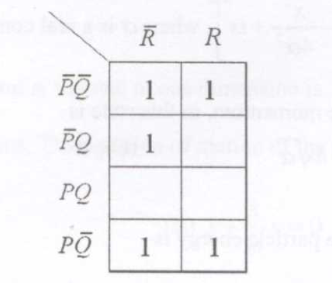
\includegraphics[width=0.3\textwidth]{figs/Q59-60fig.png}
        \captionof{figure}{Karnaugh map of a logic circuit.}
        \label{fig:q59-60}
    \end{center}

\begin{enumerate}[label=\textbf{Q. \arabic*}, start=59]

\item The minimized logic expression for the above map is
    \begin{enumerate}
    \begin{multicols}{2}
        \item $Y = \bar{P}\bar{R} + \bar{Q}$
        \item $Y = \bar{Q} \cdot PR$
        \item $Y = \bar{Q} + PR$
        \item $Y = Q \cdot \bar{P}\bar{R}$
    \end{multicols}
    \end{enumerate}
    \hfill \textbf{(GATE PH 2009)}

\item The corresponding logic implementation using gates is given as:
    \begin{enumerate}
    \begin{multicols}{2}
        \item 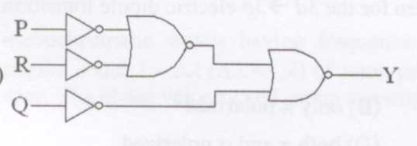
\includegraphics[width=0.9\columnwidth]{figs/Q60fig1.png}
        \item 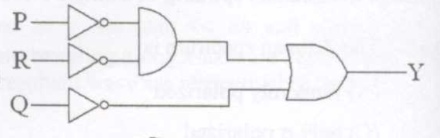
\includegraphics[width=0.9\columnwidth]{figs/Q60fig2.png}
        \item 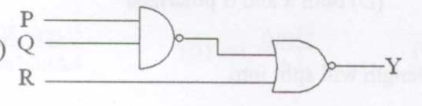
\includegraphics[width=0.9\columnwidth]{figs/Q60fig3.png}
        \item 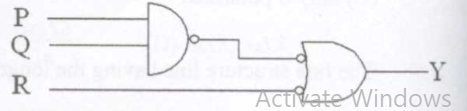
\includegraphics[width=0.9\columnwidth]{figs/Q60fig4.png}
    \end{multicols}
    \end{enumerate}
    \hfill \textbf{(GATE PH 2009)}

\end{enumerate}

\begin{center}
    \Large\textbf{END OF THE QUESTION PAPER}
\end{center}


\end{document}


